%!TEX root=../seke.tex
% mainfile: ../seke.tex

% Regression tree
% Belongs with results_trees, but must be here for page placement within the paper

\begin{figure*}[ht]
\centering
  \centering
  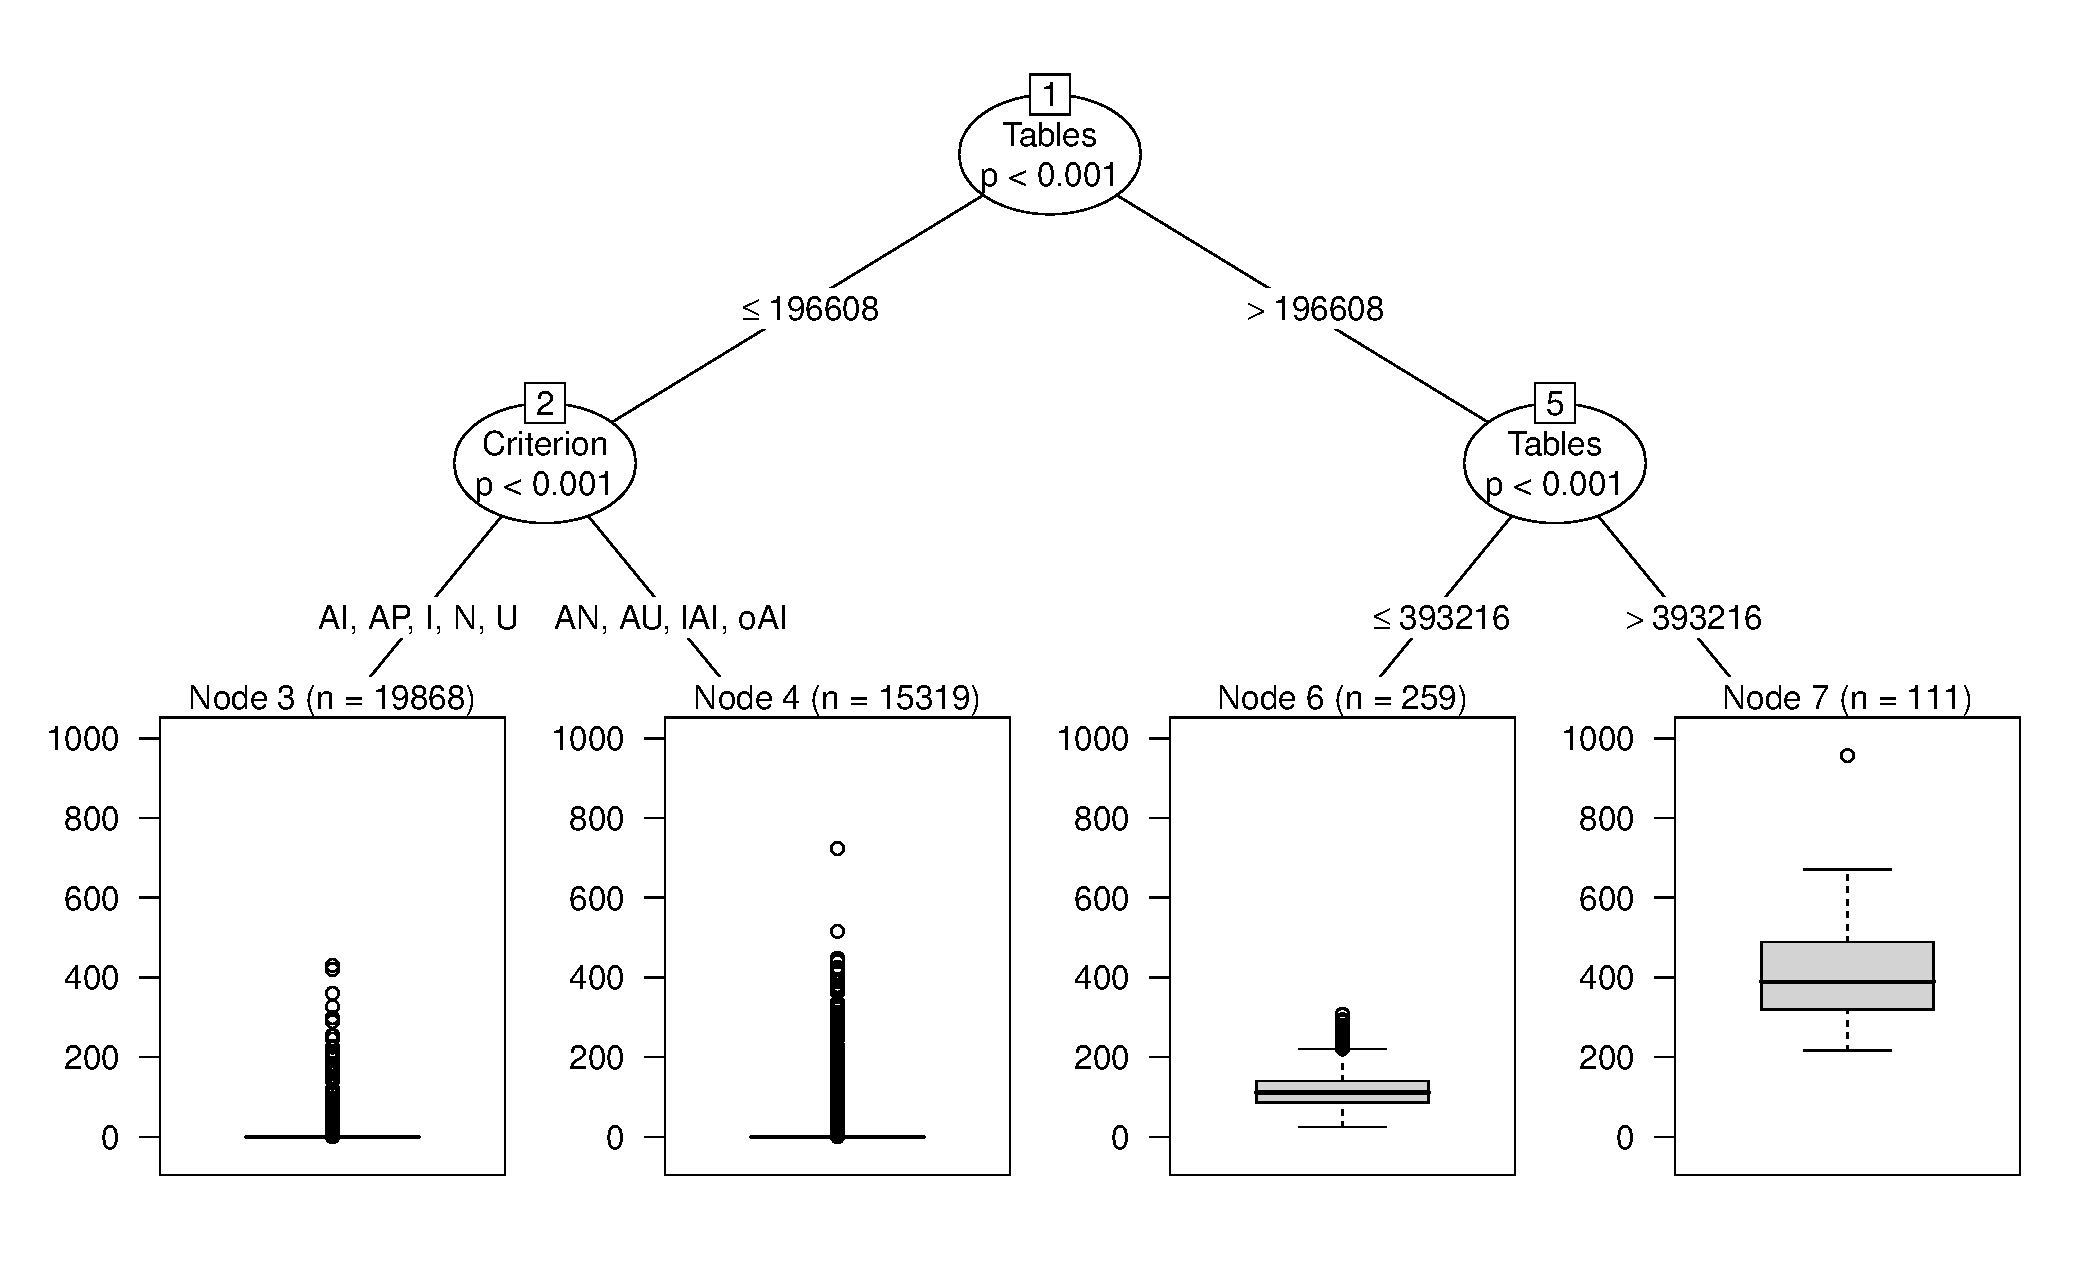
\includegraphics[width=.75\linewidth]{diagrams/AllTree.pdf}
  \caption{Regression tree using all variables to predict runtime in
  minutes. \vspace{-.15in}}
  \label{fig:atree}
\end{figure*}

\section{Empirical Analysis}

\textbf{Experimental Design}. To gain a full picture of the performance trade-offs, we conducted an experiment for every configuration
of the parameter space i.e. (schema, coverage criterion, and data generator, and doubling technique). 

In our experimental study, we set $\mathit{tolerance}$ to $0.40$ and $\mathit{lookback}$ to $4$. This value was chosen
by performing doubling experiments on various algorithms with known worst case time complexities, and observing that the
ratio converged to the correct value with this configuration.  We also conducted preliminary experiments in an attempt
to select good parameter values. We set $\mathit{minimum}$ to $20$ after observing that \textit{SchemaAnalyst} stopped
displaying constant behavior after around 5 doubles.  Preliminary studies showed that while experiments for fast
configurations could be completed in less than an hour, slower configurations required days.  Since there are over four
thousand possible configurations, the study requires a substantial amount of computational resources.  As a solution, we
conducted the experiments on a high-performance computing (HPC) cluster containing 195 worker nodes of various hardware
configurations, ranging from 12 to 16 CPU cores and 24 to 256 GB of memory, and using the 64-bit Redhat operating
system.
